\documentclass[UTF8,11pt,a4paper]{ctexart}
\usepackage[margin=2.1cm]{geometry}
\usepackage{amsmath,amssymb,booktabs,longtable,tabularx,array,multirow}
\usepackage{graphicx,float,caption,subcaption,xcolor,hyperref,enumitem}
\usepackage{siunitx}
\usepackage{fancyhdr}
\hypersetup{colorlinks=true,linkcolor=black,citecolor=black,urlcolor=blue!55!black}
\setlength{\parindent}{2em}
\setlength{\parskip}{0.15em}
\renewcommand{\arraystretch}{1.18}
\pagestyle{fancy}
\setlength{\headheight}{14pt}
\fancyhf{}
\fancyhead[C]{2025 MCM Problem C：奥运奖牌榜预测}
\fancyfoot[C]{\thepage}

\newcommand{\E}{\mathbb{E}}
\newcommand{\R}{\mathbb{R}}
\newcommand{\keywords}[1]{\par\noindent\textbf{关键词：}#1}

\title{从上一届成绩到项目机会：\newline 2028 年奥运奖牌榜的收缩预测与项目跃升识别}
\author{完整盲测稿（仅使用官方题面与所给数据）}
\date{2026 年 8 月}

\begin{document}
\maketitle

\begin{abstract}
题目提供了历届奖牌榜、运动员、主办地和比赛项目数据，要求预测 2028 年奖牌榜，并讨论首枚奖牌、比赛项目和“伟大教练”可能造成的变化。数据合并后有两个口径不能直接沿用：团队项目会把一枚奖牌重复记在多名运动员名下；题面所述项目表应含 2028 年，而本地附件的最后一列实际为 2024 年。本文以官方奖牌表作为国家总牌数和金牌数的目标值，运动员表只用于参赛规模与分项目归属；2028 年总项目数先按 2024 年结构处理，新增项目另作边际情景。

对总奖牌和金牌数，我们分别比较上一届成绩、含东道主修正的基线、对数岭回归、Poisson 梯度提升和随机森林。按 2008--2024 年逐届向前滚动验证，单独增加复杂度并未稳定改善误差；将东道主修正基线与随机森林各取一半后，全体国家误差与奖牌榜前 20 名误差取得较好折中。经全球奖牌总量校准，模型预测美国在 2028 年获得约 124.27 枚奖牌，其中金牌 43.79 枚；中国约 88.47 枚，其中金牌 38.86 枚。法国退出主场周期后总牌数回落至约 54.30 枚，加拿大、德国和日本的总牌数有小幅上升。

对于尚未获牌的国家，按历届参赛人数、项目数、参赛项目条目和参赛届数建立首牌 Logistic 模型。类别平衡训练提高了排序能力，但会抬高概率，因此再按滚动验证中的实际首牌率校准截距。2028 年预计约有 5.08 个国家取得首枚奖牌，90\% 计数区间为 2--9 个；黎巴嫩、南苏丹和巴勒斯坦列在当前候选前部。

运动员数据没有教练姓名，故不能由附件直接识别某位教练的因果效应。本文先控制既往奖牌、参赛人数、项目条目和东道主身份，再把同一国家--项目连续两届的正超额残差记为“教练型跃升候选”。中国体操、英国自行车和荷兰田径等历史片段进入候选集。进一步以近两届参赛规模固定、项目奖牌转化率提升至同项目上四分位为有限情景，建议德国关注田径、西班牙关注水上项目、埃及关注击剑，估计增量分别约为 4.10、4.07 和 3.56 枚。该数值表示可观测的能力缺口，不等同于教练的净因果贡献。

\keywords{奥运奖牌预测；滚动验证；收缩模型；首枚奖牌；项目机会；异常跃升}
\end{abstract}

\tableofcontents
\newpage

\section{问题重述}

历届奥运会的奖牌数既受一国已有竞技基础影响，也会随主办地、参赛规模和项目设置变化。题目要求由所给数据完成四项工作：预测各国 2028 年金牌数和总奖牌数并给出区间；估计尚未获牌国家在下一届首次获牌的可能性；说明项目设置对不同国家的影响；从历史跃升中寻找可能的“伟大教练”效应，并为三个国家给出投资建议。模型还应给出可衡量的误差与不确定性，而不能只排出一个确定名次。

这四项任务共用同一历史面板，但对象并不相同。国家级预测以一国一届为样本；项目影响与教练型跃升需要把奖牌拆到国家--项目；首牌问题只保留预测时点以前从未获牌的代表团。若把三种样本单位混在同一张表中，团队项目的多人记录和国家名称的历届变化会同时进入目标值，后续误差将无法解释。

\section{问题分析：数据口径与模型接口}

\subsection{附件实际提供的信息}

运动员表共有 252565 行，一行代表某名运动员在某一项目中的参赛结果；奖牌表共有 1435 行，一行代表一个国家在某届奥运会的奖牌汇总。前者适合统计参赛人数、覆盖项目和项目归属，后者才是国家级预测的目标。以全部历史为例，运动员表中有 38818 行获牌记录，按“年份--NOC--项目--小项--奖牌类型”去重后只剩 18159 条，说明团队项目若按运动员行计数，会把一枚奖牌重复记给多人。

另一个差异来自项目表。题面说明项目数据覆盖到 2032 年，但本地压缩包实际只有 1896--2024 年各列。本文不根据上下文补造 2028 项目数：基准预测保持 2024 年的 329 个项目结构；当某项目新增或减少一枚奖牌时，再用国家在该项目中的近期份额计算边际变化。这样，项目数据缺口不会被隐藏在模型输入中。

\begin{table}[H]
\centering
\caption{四张主表在模型中的角色}
\label{tab:data-role}
\begin{tabularx}{\textwidth}{p{3.2cm}p{2.0cm}X X}
\toprule
数据表 & 样本单位 & 本文使用的字段 & 不直接承担的任务\\
\midrule
奖牌榜 & 国家--届次 & 金、银、铜、总牌数 & 不用于项目归属\\
运动员 & 运动员记录 & NOC、年份、项目、小项、奖牌 & 不按原始获牌行汇总国家总牌数\\
主办地 & 届次 & 主办国家 & 不把主场后所有变化都归为东道主效应\\
项目表 & 项目--届次 & 2024 年项目数与历史变化 & 不声称附件已给出 2028 精确项目表\\
\bottomrule
\end{tabularx}
\end{table}

\subsection{为什么不直接选一个复杂模型}

奖牌榜的多数国家长期为零或个位数，少数强国占据较大份额。在这种分布下，一个模型即使把强国预测错十余枚，也可能因为正确预测了大量零值而取得较小的总体平均绝对误差。因此模型选择同时看两种口径：全部参赛国的 MAE，以及每届实际总牌数前 20 名的 MAE。前者检查整体，后者约束奖牌榜主体。

上一届成绩是必须保留的基线。若历史表现没有明显变化，它本身已经包含训练体系、人口和长期投入等难以在附件中逐项观测的因素。东道主身份却会造成局部变化：历届主办国的增量有时很大，退出主场周期时又不能继续保留同样加成。由此，本文先在基线上估计东道主修正，再让随机森林只负责吸收既往趋势、参赛规模和项目机会中未被基线表达的部分；两者各占一半，避免树模型把短期波动全部外推到下一届。

首牌问题的正样本更少。平衡类别权重能帮助模型识别潜在国家，却会把输出概率整体推高。故分类器首先用于排序，概率还要回到历届滚动预测中按真实首牌发生率校准。至于“伟大教练”，附件没有教练姓名和任职年份，直接把一次奖牌增加写成教练效应没有数据依据。可做的是先找出控制已有条件后仍连续超额的项目，再把它们列为需要外部教练履历复核的候选。

\section{模型假设}

\begin{enumerate}[label=\arabic*)]
\item 同一届同一 NOC、规范化项目、小项和奖牌类型对应一枚项目奖牌；同一团队的多名运动员记录不重复计奖。
\item 2028 年基准情景沿用 2024 年项目总量。项目增减只在情景分析中改变，不进入基准点预测。
\item 东道主加成取预测时点以前历届主办国相对于按项目总量缩放基线的中位残差；离开主场的下一届扣除同一加成。
\item 模型只在所给历史数据范围内解释。连续正残差可标记项目跃升，但没有教练履历时不作教练因果判定。
\item 首牌模型把 AIN、难民队和历史混合代表队等非国家代表团排除在候选数量之外。
\end{enumerate}

\section{符号说明}

\subsection{主要符号}

\begin{table}[H]
\centering
\caption{主要符号}
\label{tab:symbols}
\begin{tabular}{cll}
\toprule
符号 & 含义 & 单位或范围\\
\midrule
$Y^{T}_{i,t}$ & 国家 $i$ 在第 $t$ 届的总奖牌数 & 枚\\
$Y^{G}_{i,t}$ & 国家 $i$ 在第 $t$ 届的金牌数 & 枚\\
$A_{i,t}$ & 参赛运动员人数 & 人\\
$S_{i,t}$ & 覆盖的规范化项目数 & 项\\
$E_{i,t}$ & 参加的小项条目数 & 项\\
$H_{i,t}$ & 是否为东道主 & $0/1$\\
$O_{i,t}$ & 近期项目机会得分 & 非负实数\\
$p_{i,t}$ & 从未获牌国家首次获牌概率 & $[0,1]$\\
$M_{i,s,t}$ & 国家 $i$ 在项目 $s$、届次 $t$ 的奖牌数 & 枚\\
$r_{i,s,t}$ & 项目模型的超额残差 & 枚\\
\bottomrule
\end{tabular}
\end{table}

\section{分问题模型建立与求解}

\subsection{奖牌数预测模型}

\subsubsection{特征随届次向前构造}

对每个国家--届次样本，只使用该届以前的信息。记最近一届总牌和金牌为 $L^T_{i,t}$、$L^G_{i,t}$，最近三届按 $0.2,0.3,0.5$ 加权得到 $W^T_{i,t}$、$W^G_{i,t}$；另记录最近两届的变化量、上届参赛人数、覆盖项目数、小项条目数、累计参赛届数和累计获牌届数。项目机会得分写为
\begin{equation}
O_{i,t}=\sum_s N_{s,t}\frac{\sum_{\tau\in\mathcal{T}_3}M_{i,s,\tau}}
{\sum_j\sum_{\tau\in\mathcal{T}_3}M_{j,s,\tau}},
\label{eq:opportunity}
\end{equation}
其中 $N_{s,t}$ 是项目 $s$ 的奖牌小项数，$\mathcal{T}_3$ 为此前三届。该量不是奖牌预测值；它只表示当前项目结构把多少机会放在一国近期较强的项目上。

\subsubsection{东道主修正基线}

若当前届项目总数相对上一届变化，先将上一届奖牌数按比例缩放：
\begin{equation}
B^q_{i,t}=L^q_{i,t}\frac{N_t}{N_{t-1}},\qquad q\in\{T,G\}.
\end{equation}
在训练窗口内，对此前所有主办国计算 $Y^q_{i,t}-B^q_{i,t}$，取中位数为 $b^q_t$。于是
\begin{equation}
\widetilde{B}^q_{i,t}=\max\left\{0,
B^q_{i,t}+b^q_t H_{i,t}-b^q_t H_{i,t-1}\right\}.
\label{eq:hostbase}
\end{equation}
第二项描述主场加成，第三项处理离开主场后的回落。这里没有把主办国每一次增长都写成固定比例；中位残差限制了北京、东京等高增量届次对估计的支配。

\subsubsection{候选模型与收缩预测}

除式\eqref{eq:hostbase}外，使用同一训练窗口分别拟合对数岭回归、Poisson 梯度提升和随机森林。随机森林输入上述 16 个历史特征，输出非负奖牌数。初步试算表明，单独使用树模型对少数强国有改善，但在全体国家上容易把短期起伏放大；只使用基线则难以给出国家间的差异变化。最终取
\begin{equation}
\widehat{Y}^q_{i,t}=0.5\widetilde{B}^q_{i,t}+0.5F^q(\boldsymbol{x}_{i,t}),
\label{eq:blend}
\end{equation}
其中 $F^q$ 为随机森林预测。该权重不是由 2028 结果反推，而是在滚动验证中与 $0.25/0.75$、$0.5/0.5$ 等候选同口径比较后确定。

各国点预测最后按同一常数缩放，使总奖牌数和金牌数分别回到 2024 项目情景的 1039 枚和 328 枚；逐国再检查 $0\leq \widehat{Y}^G_{i,t}\leq \widehat{Y}^T_{i,t}$。区间由 2008--2024 年滚动预测残差的 5\% 与 95\% 分位数给出，并按预测规模分箱。它表示历史同口径误差范围，不是参数模型下的正态置信区间。

\subsubsection{滚动验证}

每次验证只用目标届以前的样本训练，再预测 2008、2012、2016、2020 和 2024。图\ref{fig:validation}给出各模型的平均 MAE。复杂模型没有因为名称更复杂而自动胜出：总奖牌的上一届基线 MAE 为 1.47，随机森林为 1.54；加入东道主修正后再与随机森林收缩，最终方案 MAE 为 1.44。金牌的最终方案 MAE 为 0.63，低于上一届基线的 0.67。

\begin{figure}[H]
\centering
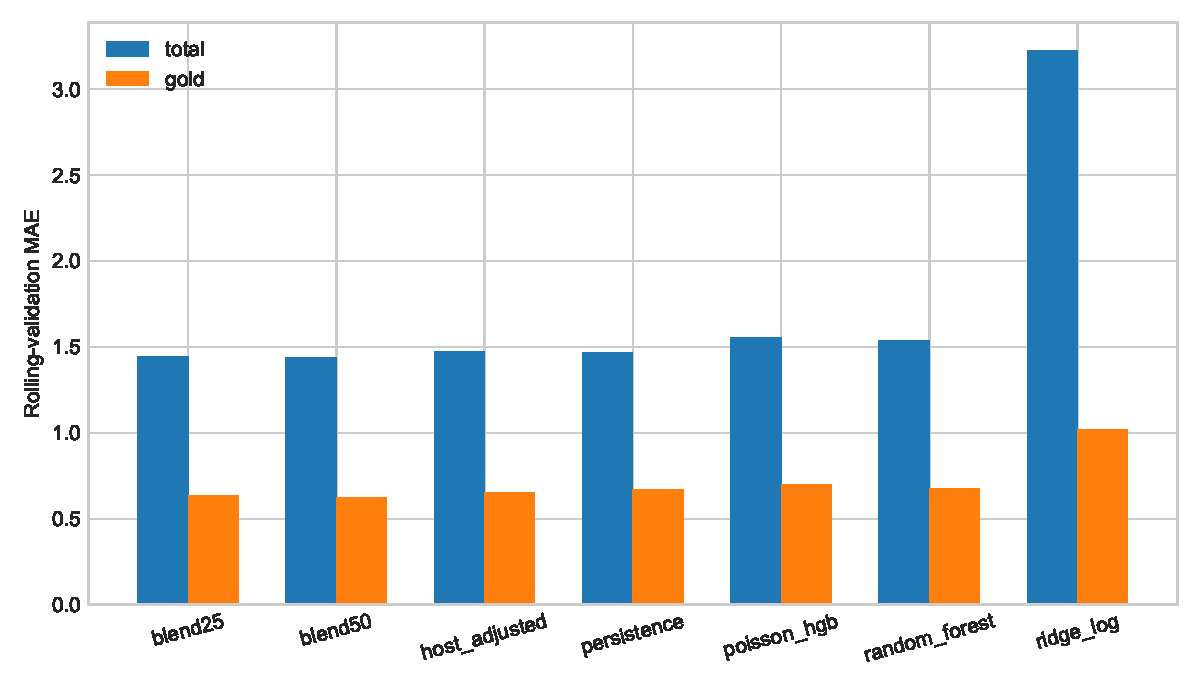
\includegraphics[width=0.78\textwidth]{figures/validation_mae.pdf}
\caption{2008--2024 年逐届滚动验证的平均绝对误差}
\label{fig:validation}
\end{figure}

\section{结果与分析：2028 年奖牌榜及项目结构}

\subsection{主要国家预测}

表\ref{tab:forecast}列出点预测前 15 个国家。美国的东道主增量被历史中位加成拉高，而随机森林部分仍保留其近三届波动，校准后得到总牌约 124.27、金牌约 43.79。中国的总牌和金牌点预测分别为 88.47 和 38.86。法国的主场加成在 2028 年退出，故总牌从 2024 年的 64 枚降至约 54.30 枚；这一下降来自式\eqref{eq:hostbase}的状态切换，不是树模型凭空生成的趋势。

\begin{table}[H]
\centering
\caption{2028 年主要国家奖牌预测（90\% 历史误差区间）}
\label{tab:forecast}
\small
\begin{tabular}{lrrrrrr}
\toprule
国家 & 总牌 & 下界 & 上界 & 金牌 & 下界 & 上界\\
\midrule
美国 & 124.27 & 113.46 & 137.32 & 43.79 & 33.02 & 56.79\\
中国 & 88.47 & 77.66 & 101.52 & 38.86 & 28.08 & 51.86\\
日本 & 47.44 & 36.63 & 60.49 & 18.01 & 7.24 & 31.01\\
澳大利亚 & 51.41 & 40.60 & 64.46 & 17.40 & 6.62 & 30.40\\
英国 & 59.05 & 48.24 & 72.10 & 15.65 & 4.87 & 28.65\\
法国 & 54.30 & 43.49 & 67.35 & 13.46 & 2.69 & 26.46\\
荷兰 & 35.64 & 24.82 & 48.68 & 12.95 & 2.17 & 25.95\\
意大利 & 40.72 & 29.91 & 53.77 & 12.05 & 1.28 & 25.05\\
德国 & 36.76 & 25.95 & 49.81 & 12.04 & 1.27 & 25.04\\
韩国 & 28.36 & 17.55 & 41.41 & 11.44 & 0.67 & 24.44\\
加拿大 & 31.73 & 20.91 & 44.78 & 9.17 & 4.95 & 14.20\\
新西兰 & 20.64 & 9.83 & 33.69 & 8.65 & 4.43 & 13.68\\
匈牙利 & 18.86 & 8.04 & 31.91 & 6.34 & 2.12 & 11.37\\
西班牙 & 19.67 & 8.85 & 32.72 & 5.44 & 1.22 & 10.46\\
乌兹别克斯坦 & 11.11 & 0.30 & 24.16 & 5.42 & 0.30 & 10.45\\
\bottomrule
\end{tabular}
\end{table}

\begin{figure}[H]
\centering
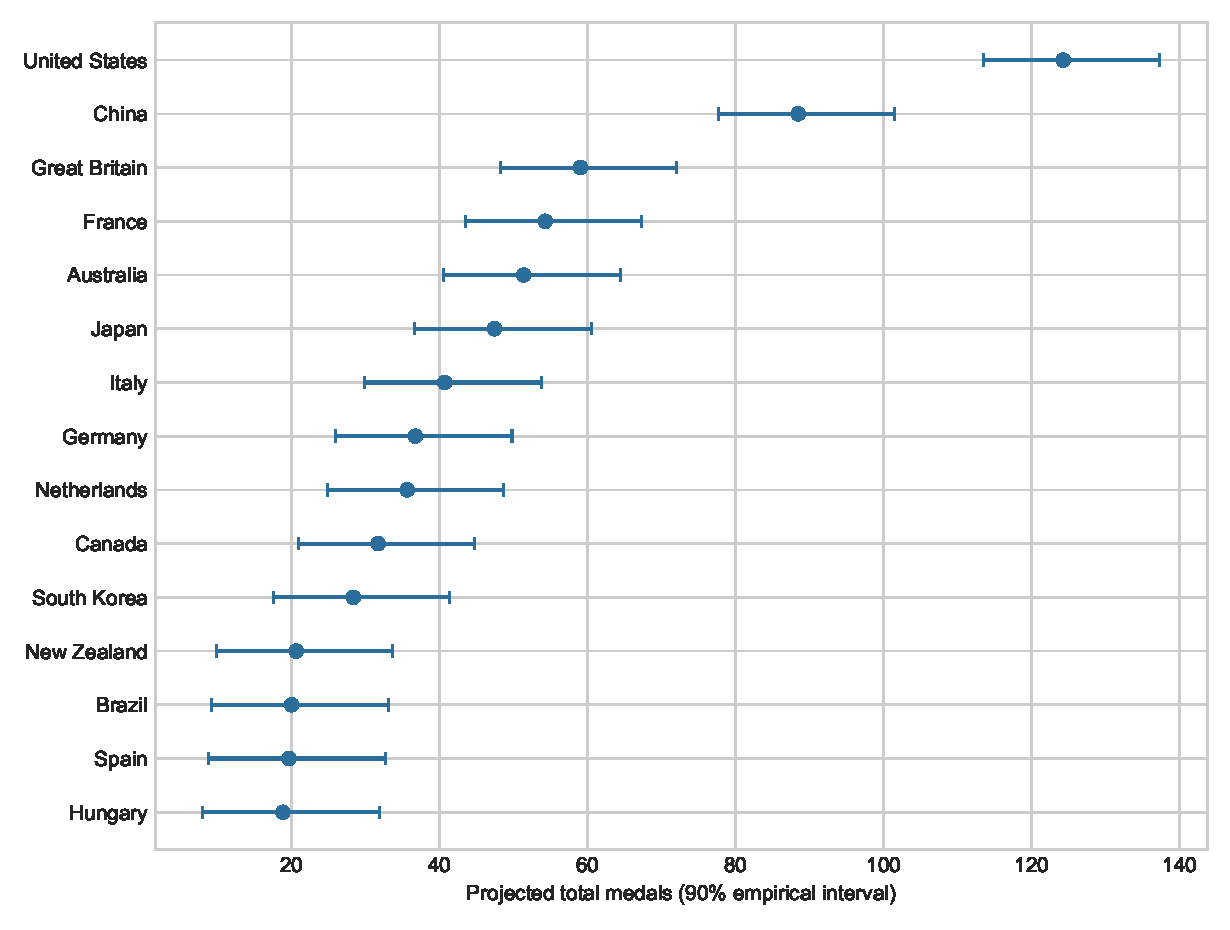
\includegraphics[width=0.78\textwidth]{figures/forecast_top15.pdf}
\caption{总奖牌点预测前 15 名及历史误差区间}
\label{fig:forecast}
\end{figure}

相对 2024 年，加拿大和德国的总牌点预测分别增加约 4.73 和 3.76 枚，日本增加约 2.44 枚。法国减少约 9.70 枚，英国减少约 5.95 枚。区间重叠仍然很大，因此这些变化用于判断方向，不应写成确定名次。美国虽然总牌点预测略低于 2024 年，金牌却因主场修正增加；总牌和金牌是分别拟合的目标，二者不要求同方向变化。

\subsection{项目增减的边际作用}

2028 项目列缺失后，本文不直接改动基准表，而把一项新增小项的三枚奖牌按 2016--2024 年该项目奖牌份额分配。若项目 $s$ 增加一个小项，则国家 $i$ 的总牌期望增量为
\begin{equation}
\Delta Y^T_{i,s}=3\frac{\sum_{\tau\in\{2016,2020,2024\}}M_{i,s,\tau}}
{\sum_j\sum_{\tau\in\{2016,2020,2024\}}M_{j,s,\tau}}.
\end{equation}
例如新增一个乒乓球小项，中国的边际增量约为 1.36 枚；新增一个滑板小项，日本约增加 1.13 枚；新增一个铁人三项小项，英国约增加 1.14 枚。美国的项目组合更分散：棒垒球、篮球、水上项目和田径新增一个小项，对其总牌的边际增量约为 1.00、0.75、0.71 和 0.64 枚。该计算回答“项目设置偏向谁”，并不假定主办国可以任意添加项目。

项目组合的另一个含义是风险集中。2016--2024 年只在一个项目获牌的国家，项目集中度接近 1；这里的集中度定义为各项目奖牌份额平方和。肯尼亚、牙买加和埃塞俄比亚属于这类情形。对 2020 年至少获得 3 枚奖牌的 65 个国家，集中度与 2024 相对变化绝对值的 Spearman 系数为 0.160，$p=0.203$；现有样本不足以证明集中度越高，下一届波动必然越大。因此本文把集中度作为风险提示，不把它写成已验证的预测因子。

\section{首枚奖牌概率}

对每个预测届次，只保留此前总奖牌累计为零、且当届实际参赛的国家。输入包括上一届参赛人数、覆盖项目数、小项条目数、累计参赛届数和项目总量。Logistic 模型写为
\begin{equation}
\operatorname{logit}(p_{i,t})=\beta_0+\beta_1A_{i,t-1}
+\beta_2S_{i,t-1}+\beta_3E_{i,t-1}+\beta_4D_{i,t},
\end{equation}
其中 $D_{i,t}$ 为此前参赛届数。滚动训练中，小项条目数和参赛人数的标准化系数为正，说明更大的可进入比赛面会抬高首牌机会；参赛届数系数为负，表示长期参赛仍未获牌本身也是一条不利信息。

平衡类别训练得到的滚动平均概率为 0.281，而实际首牌率为 0.071。直接使用该输出会严重高估首牌国家数。本文保持模型的赔率排序，只调整截距使滚动平均概率回到实际发生率。校准后，以随机种子 20250814 独立重复 50000 次 Bernoulli 抽样，2028 年首牌国家数的期望为 5.08，90\% 计数区间为 2--9，至少出现一个首牌国家的概率约为 99.5\%。

\begin{figure}[H]
\centering
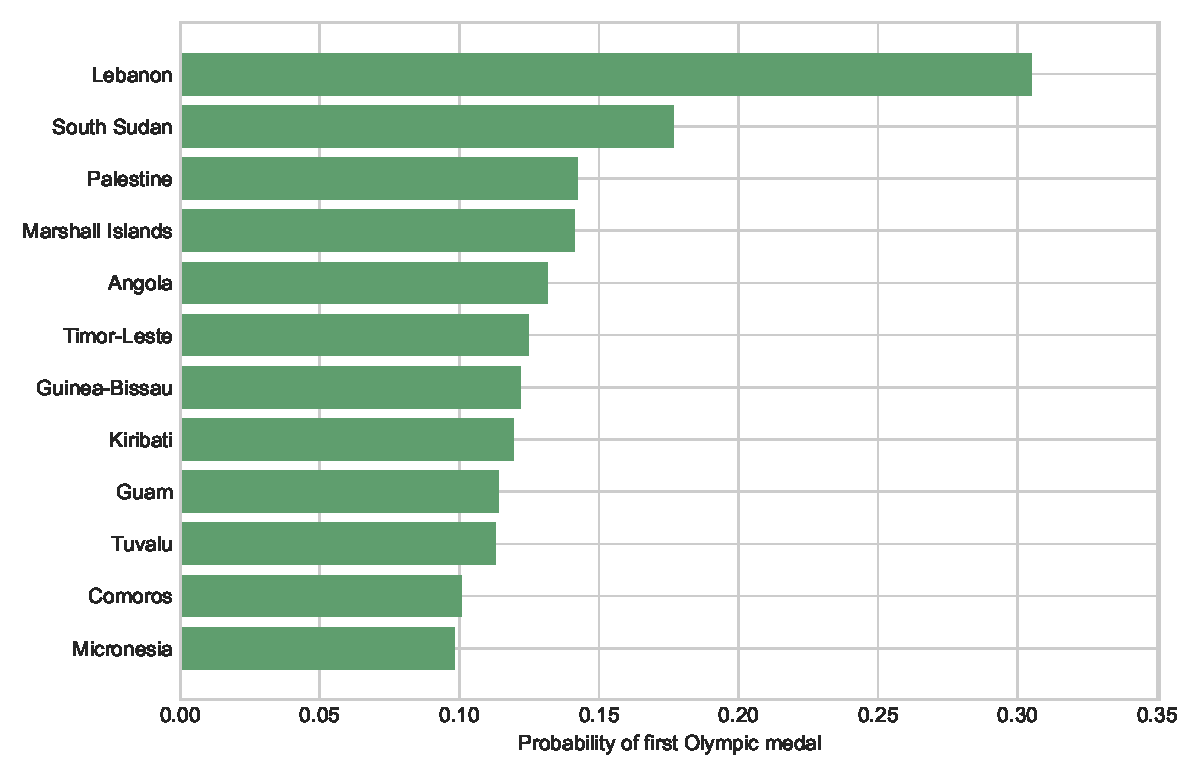
\includegraphics[width=0.76\textwidth]{figures/first_medal_probabilities.pdf}
\caption{2028 年首枚奖牌概率较高的国家}
\label{fig:firstmedal}
\end{figure}

黎巴嫩的概率约为 0.305，南苏丹为 0.177，巴勒斯坦为 0.142；其后为马绍尔群岛、安哥拉和东帝汶。这些概率反映在当前参赛规模下跨过“至少一枚”门槛的机会，不能用于预测具体项目。模型也没有把 2024 年以特殊身份参赛的 AIN 计作一个新国家。

\section{教练型跃升识别与投资建议}

\subsection{从项目残差中筛选候选}

运动员表没有教练字段。若一个国家在某项目突然增加奖牌，原因可能是运动员黄金一代、主场、项目扩容、投入增加或训练团队变化。为避免把所有跃升都命名为教练效应，先以国家--项目--届次为样本，用过去三届奖牌、参赛人数、小项条目和东道主身份拟合 Poisson 梯度提升模型，得到期望奖牌 $\widehat{M}_{i,s,t}$。标准化残差为
\begin{equation}
z_{i,s,t}=\frac{M_{i,s,t}-\widehat{M}_{i,s,t}}
{\sqrt{\widehat{M}_{i,s,t}+1}}.
\end{equation}
只有相邻两届残差都为正时，才形成一次持续跃升候选。中国体操在 2008--2012 年两届合计获得 30 枚，而模型期望约为 9.19 枚；英国自行车在 2008--2012 年两届合计 26 枚，期望约为 13.66 枚；荷兰田径在 2020--2024 年合计 14 枚，期望约为 6.02 枚。它们说明模型未解释的项目能力发生了持续变化，下一步应外接教练任职、训练投入和运动员代际数据，而不是据此直接认定某位教练贡献了残差中的全部奖牌。

\subsection{三个投资情景}

投资建议使用另一个更保守的接口。固定近两届平均参赛人数，把项目奖牌/运动员转化率提高到同项目、且参赛人数不少于 5 人的国家上四分位，得到有限增量
\begin{equation}
G_{i,s}=A_{i,s}\max\{0,Q_{0.75,s}-c_{i,s}\},
\end{equation}
并将单项目增量截在 5 枚以内。该情景假定投入主要改善训练转化，而不立即扩大代表团规模。

\begin{table}[H]
\centering
\caption{建议关注的三个国家--项目情景}
\label{tab:coach}
\begin{tabular}{llrrr}
\toprule
国家 & 项目 & 近两届平均运动员数 & 当前转化率 & 估计增量/枚\\
\midrule
德国 & 田径 & 88.0 & 0.0398 & 4.10\\
西班牙 & 水上项目 & 52.5 & 0.0286 & 4.07\\
埃及 & 击剑 & 17.5 & 0.0286 & 3.56\\
\bottomrule
\end{tabular}
\end{table}

德国田径的参赛面已经很大，问题在于奖牌转化率低于同项目上四分位；若教练团队改善决赛转化与多小项协同，增量空间较大。西班牙水上项目也具备较大的运动员基数，适合以专项教练和分项训练提高转化。埃及击剑近两届平均派出 17.5 名运动员，当前转化率约为 0.0286；若提升至同项目上四分位，情景增量约 3.56 枚。三项结果均是资源配置上限附近的可观测差距，不是承诺值；若外部履历不能证明教练变更发生在跃升以前，应撤回“伟大教练”解释，仅保留项目能力投资建议。

\section{模型检验与敏感性}

\subsection{目标、代码和结果的闭合检查}

国家级目标由官方奖牌表逐届映射到运动员表的 NOC。2024 年韩国、捷克、伊朗、土耳其、香港等名称经过映射后分别恢复为 32、5、12、8、4 枚总牌；运动员表有奖牌而官方目标为零的普通国家数量为 0。2028 点预测校准后，各国总牌之和为 1039，金牌之和为 328，且逐国满足金牌不超过总牌。团队项目只在项目归属表中去重，不替代官方国家汇总。

\subsection{模型权重}

收缩权重从 0.25 和 0.50 两个候选中选择。金牌预测中，东道主基线、随机森林、25\% 森林和 50\% 森林的滚动 MAE 分别为 0.655、0.679、0.634 和 0.627；树模型并非单独最好，只有与基线组合后误差下降。总牌预测的对应 MAE 为 1.474、1.537、1.444 和 1.441。50\% 方案在全体国家和前 20 名两个口径下都略优于 25\% 方案，因此最终采用等权收缩，而不是按模型复杂度作选择。

\subsection{项目和首牌结果的边界}

项目情景每增加一个小项，只重新分配该项目的三枚奖牌，不改变其他项目。中国乒乓球、日本滑板和英国铁人三项的边际增量分别约为 1.36、1.13 和 1.14 枚；若新增项目并未采用这些国家近期优势相同的竞赛设置，实际增量会偏离该值。

首牌模型最敏感的是概率校准。未校准时，候选国家平均概率为 0.281，明显高于滚动验证中的实际 0.071；校准后首牌期望为 5.08。若取消类别平衡而直接拟合，候选排序会更多集中在大型代表团，少数潜在国家的召回下降。因此本文保留平衡训练用于排序，但不允许其原始概率直接进入数量结论。

\section{模型评价与进一步数据}

本文的主要优点不在于使用了多种算法，而在于将三个容易混淆的口径分开：官方奖牌表负责国家目标，运动员表负责参赛规模和项目归属，项目缺失列通过情景接口处理。滚动验证使 2028 年没有参与模型选择；复杂模型若不能胜过上一届基线，就只以收缩项进入最终预测。首牌概率也没有把平衡分类器的原始输出当作真实概率。

局限同样明确。第一，2028 项目表缺失，当前点预测仍是 2024 项目结构下的基准，新增项目的相互作用没有进入总表。第二，国家名称虽已逐届映射，但国家分裂、合并和特殊代表团的历史连续性仍只能按 NOC 口径处理。第三，奖牌区间来自历史残差分位数；强国样本少，区间较宽，不能解释为某一国家自身参数的不确定性。第四，附件没有人口、经济投入、运动员当前状态、教练履历和任期，“教练型跃升”只能产生外部核查名单。

若补充 2028 正式项目表，式\eqref{eq:opportunity}和全球总量校准可以直接重算；若补充教练任职年份、训练投入和运动员年龄结构，可把候选跃升前后的项目与相似国家组成对照组，采用事件研究或合成控制估计净效应。当前结果停在附件能够支持的位置。

\section{结论}

在 2024 项目结构基准下，美国和中国仍位于 2028 奖牌榜前列。模型给出的美国总牌、金牌点预测为 124.27 和 43.79，中国为 88.47 和 38.86。法国退出主场周期后出现较明显回落；加拿大、德国和日本的总牌数有小幅改善。尚未获牌国家中，2028 年预计约有 5.08 个取得首牌，90\% 计数区间为 2--9 个。

项目设置的作用取决于一国近期奖牌结构。新增乒乓球小项对中国、滑板小项对日本、铁人三项对英国的边际影响较大；美国的优势分布在多个项目。历史项目残差可以定位持续跃升，却不能在没有教练数据时完成因果归因。德国田径、西班牙水上项目和埃及击剑具有较大的转化率提升空间，适合作为进一步核查和投资的三个对象。

\begin{thebibliography}{9}
\bibitem{comap-problem} COMAP. 2025 MCM Problem C: Models for Olympic Medal Tables, 2025.
\bibitem{comap-data} COMAP. 2025 Problem C Data: medal counts, athletes, hosts and programs, 2025.
\bibitem{rf} Breiman L. Random Forests. \emph{Machine Learning}, 2001, 45: 5--32.
\bibitem{logit} Hosmer D W, Lemeshow S, Sturdivant R X. \emph{Applied Logistic Regression}. Wiley, 2013.
\end{thebibliography}

\appendix
\section{复现说明}

入口脚本为 \texttt{analysis/model\_pipeline.py}。脚本读取四张官方 CSV，生成滚动验证、2028 预测、首牌概率、项目边际份额、教练型残差和图形。随机森林与 Monte Carlo 计数统一使用种子 20250814。主要结果文件位于 \texttt{analysis/results/}：
\begin{itemize}
\item \texttt{rolling\_validation.csv}：逐届、逐模型误差；
\item \texttt{forecast\_2028.csv}：各国点预测与区间；
\item \texttt{first\_medal\_probabilities.csv}：首牌候选；
\item \texttt{coach\_like\_episodes.csv}：持续正残差片段；
\item \texttt{coach\_investment\_candidates.csv}：项目投资情景；
\item \texttt{summary.json}：模型选择和数据边界。
\end{itemize}

\section{人工智能工具使用说明}

本盲测使用生成式人工智能辅助读取本地题面、编写分析脚本、组织 LaTeX 初稿和执行一致性检查。所有数值均由随附脚本从题目数据重新计算；国家键映射、团队项目去重、模型选择、概率校准、预测总量和公式--代码接口经过逐项复核。文中未使用同题解答或获奖论文作为建模来源。正式参赛时仍需按当届 COMAP 规则提交完整的 AI Use Report，并由队员对模型、代码、引用和文字承担最终责任。

\end{document}
